\documentclass[conference]{IEEEtran}

\usepackage{cite}
\usepackage{amsmath,amssymb,amsfonts}
\usepackage{graphicx}
\usepackage{textcomp}
\usepackage{xcolor}
\usepackage{url}

\title{Comparing Equivariant and Non-Equivariant VAE Representations for Semi-Supervised Histopathology WSI Classification}

\author{
\IEEEauthorblockN{Maximiliano Garavito Chtefan}
\IEEEauthorblockA{
Escuela de Ingenieria de Sistemas e Informatica\\
Universidad Industrial de Santander\\
Bucaramanga, Colombia\\
email pending}
\and
\IEEEauthorblockN{David Romo Bucheli}
\IEEEauthorblockA{
Escuela de Ingenieria de Sistemas e Informatica\\
Universidad Industrial de Santander\\
Bucaramanga, Colombia\\
email pending}
}

\begin{document}

\maketitle

\begin{abstract}
This paper studies a semi-supervised pipeline for histopathology whole-slide
image classification. The practical problem is simple: unlabeled patches are
available in large quantities, while expert labels are expensive and slow to
produce. We therefore first train a denoising variational autoencoder on
unlabeled histopathology patches and then use the encoder embeddings to train a
WSI-level classifier with limited supervision. The planned comparison keeps the
data, objective, latent size, classifier protocol, and evaluation fixed while
changing the encoder family: a translatable non-equivariant convolutional VAE
versus a continuous rotation-equivariant $\mathrm{SO}(2)$ VAE. This scaffold
records the experimental plan and paper structure; quantitative results remain
pending until the Kaggle runtime selection, full VAE runs, equivariant model,
and downstream classifier experiments are complete.
\end{abstract}

\begin{IEEEkeywords}
histopathology, whole-slide image classification, semi-supervised learning,
variational autoencoder, rotation equivariance, $\mathrm{SO}(2)$
\end{IEEEkeywords}

\section{Introduction}

Digital pathology makes it possible to analyze whole-slide images (WSIs) with
computational methods, but it does not remove the central bottleneck of expert
annotation. In cancer pathology, the diagnostic process is costly, time
consuming, and affected by high visual variability between tissue samples and
between observers. Deep learning can help with this problem, but fully
supervised models need many labeled examples, and those labels are precisely
the expensive part of the pipeline \cite{litjens_survey_2017,song_artificial_2023,baxi_digital_2022}.

The working idea of this paper follows the thesis direction: use the unlabeled
images first. A VAE-style encoder is trained without WSI labels by reconstructing
or denoising histopathology patches. After this unsupervised step, the learned
embeddings are used by a classifier trained with the available WSI labels. The
question is whether a rotation-aware encoder gives better representations than
a comparable ordinary convolutional encoder.

Histopathology patches usually do not have a preferred orientation. If a tissue
structure is rotated in the slide, the biological content is still the same
structure. Ordinary CNNs already exploit translation equivariance, but rotation
equivariance must be added by architecture or learned indirectly from data. This
paper targets continuous $\mathrm{SO}(2)$ equivariance because the scientific
question is about rotation structure, not only about a small discrete set of
right-angle rotations.

\begin{figure*}[t]
\centering
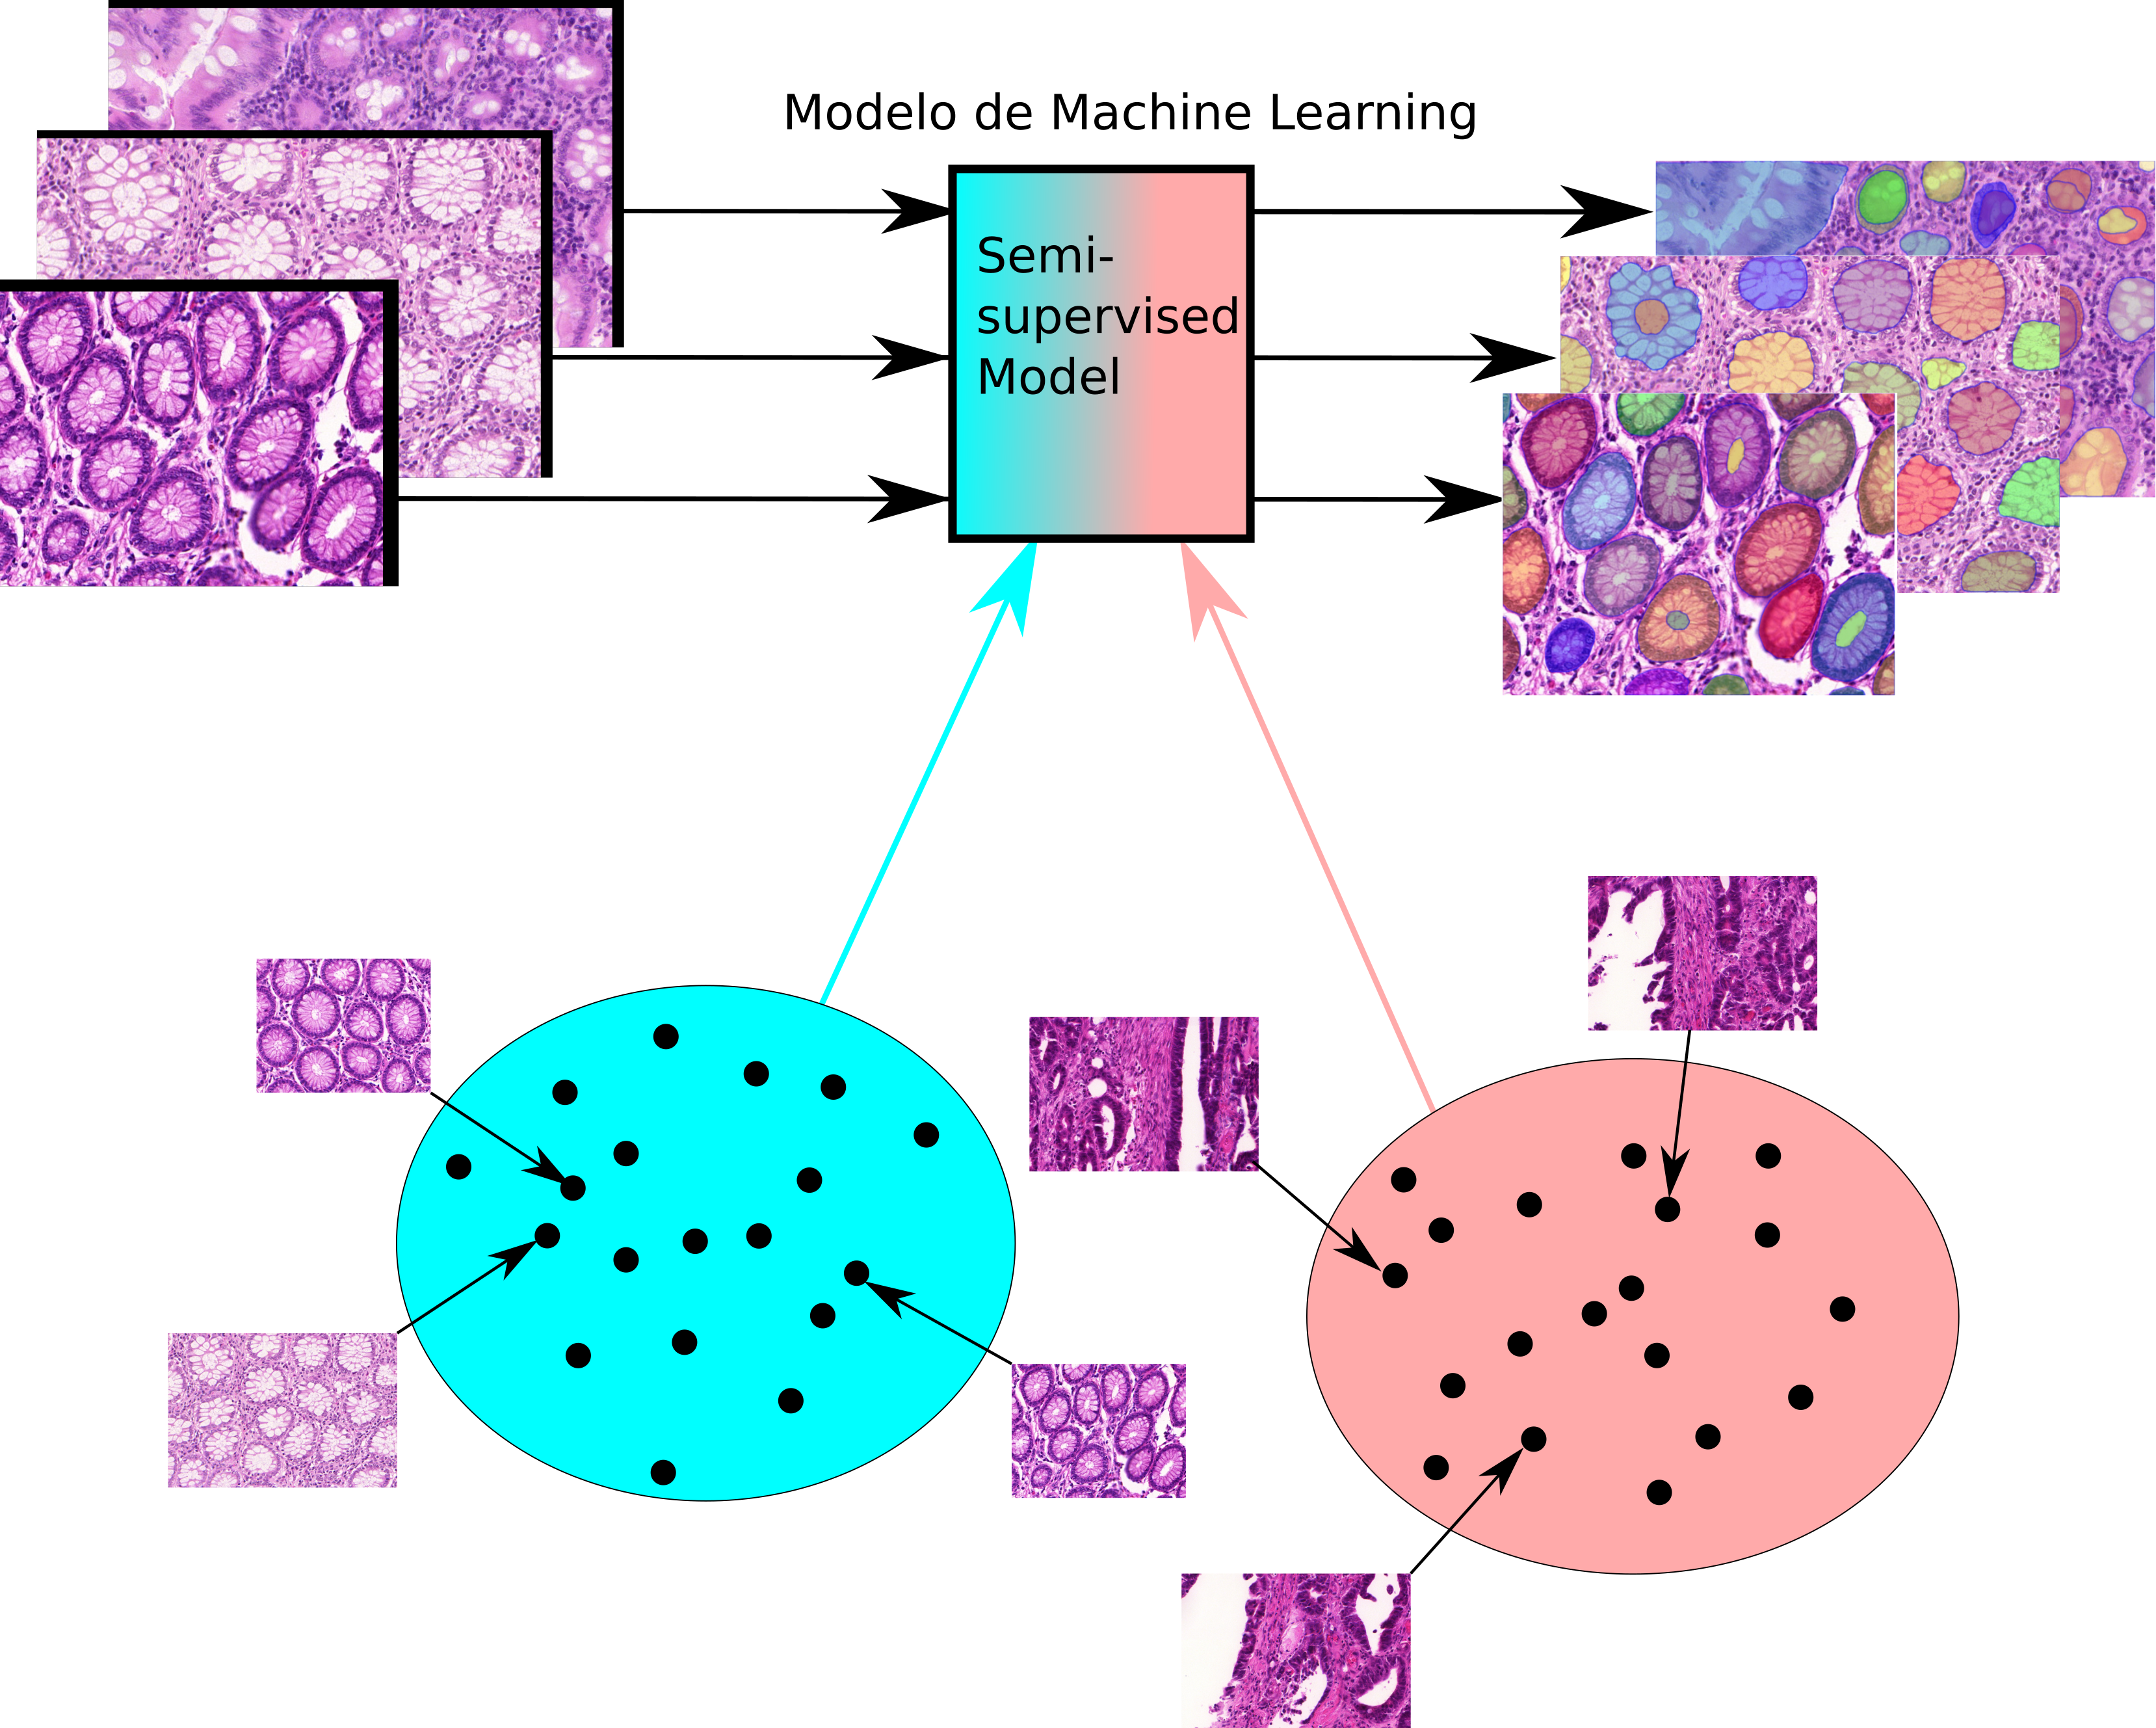
\includegraphics[width=0.85\textwidth]{figures/semi_supervised_model.png}
\caption{Semi-supervised learning idea reused from the thesis material. The
paper version will formalize this as an unsupervised VAE representation step
followed by a supervised WSI classifier trained on encoder embeddings. This
draft figure is a scaffold and may be redrawn before submission.}
\label{fig:semi-supervised-pipeline}
\end{figure*}

\section{Background and Related Work}

\subsection{Histopathology Representation Learning}

WSI analysis is different from ordinary image classification because a single
slide is too large to process directly at full resolution. A common strategy is
to work with patches or compressed representations and then aggregate local
evidence at the slide level. Tellez et al. proposed neural image compression for
gigapixel histopathology, where an unsupervised representation is learned before
weakly supervised prediction \cite{tellez_neural_2021}. This is close to the
basic structure used here: learn useful patch embeddings first, and ask the
classifier to solve the label problem with a smaller supervised burden.

\subsection{Equivariant Neural Networks}

Equivariant CNNs encode known symmetries into the model instead of asking the
network to rediscover them from data. Group-equivariant CNNs and steerable CNNs
formalize this idea through feature fields and equivariant convolutional kernels
\cite{cohen_group_2016,cohen_steerable_2016}. The general motivation is that
when the target task respects a symmetry, using that symmetry can reduce sample
complexity and improve generalization \cite{elesedy_provably_2021}. In digital
pathology, rotation-equivariant CNNs have already been studied because tissue
orientation is often not semantically fixed \cite{veeling_rotation_2018}.

\begin{figure}[t]
\centering
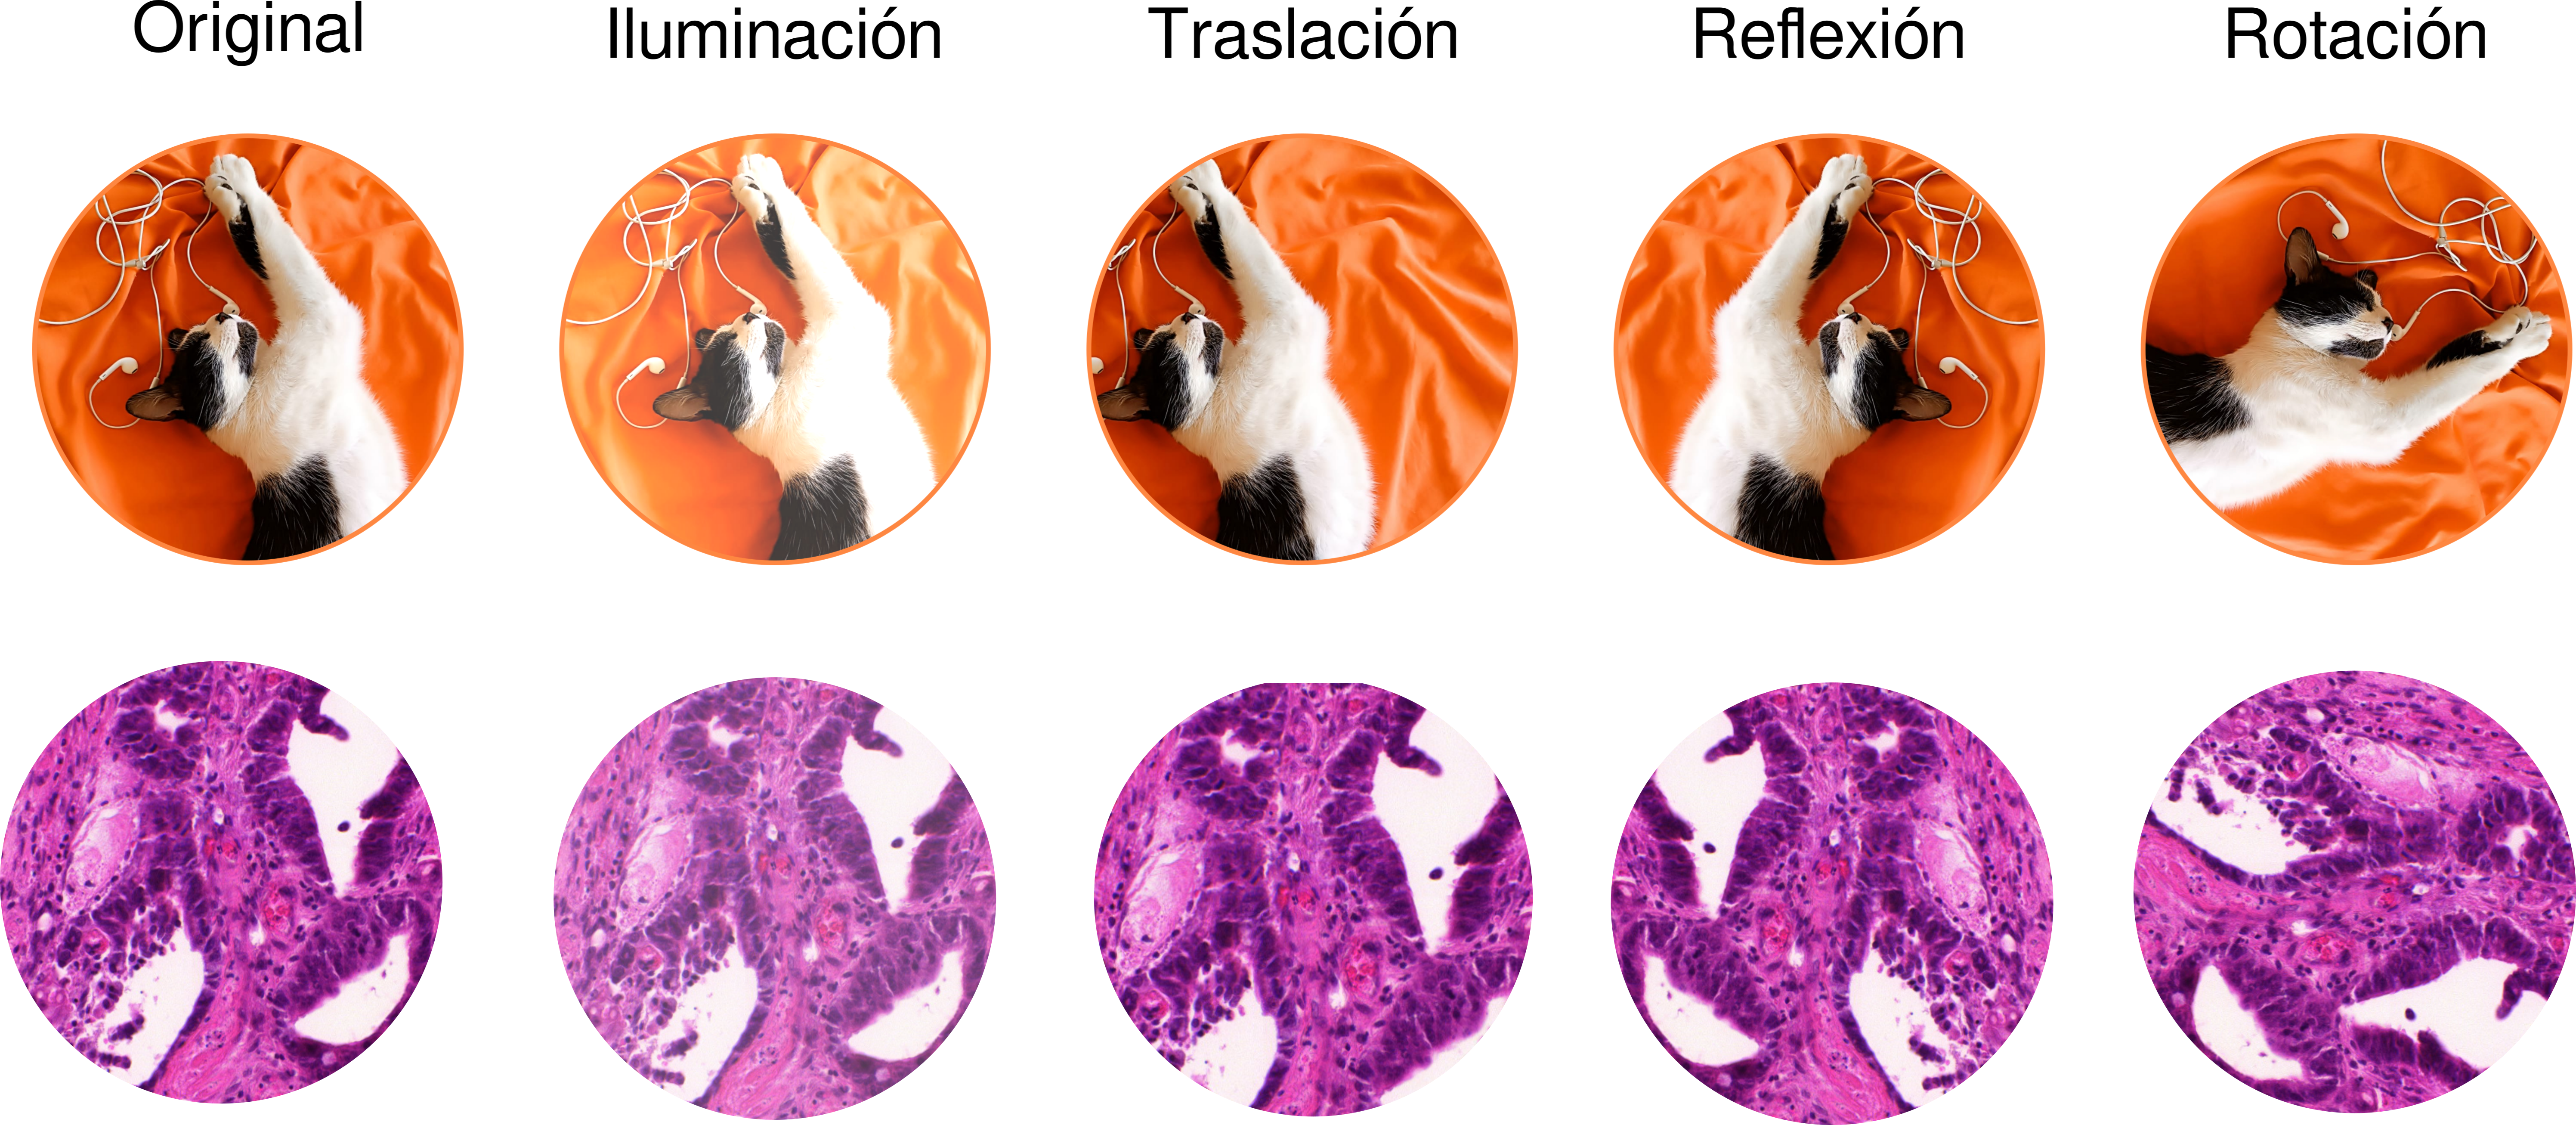
\includegraphics[width=\linewidth]{figures/transformaciones_gato_wsi.png}
\caption{Rotation intuition from the thesis figures. The histopathology patch
keeps its tissue content under rotation, unlike examples where orientation can
change the class semantics. The final paper figure should focus only on the
histopathology row.}
\label{fig:rotation-intuition}
\end{figure}

\subsection{Variational Autoencoders}

The representation learner in this work is a normal denoising VAE, not the
historical FSQ autoencoder used in earlier engineering experiments. The encoder
produces $\mu$ and $\log \sigma^2$, samples a latent representation with the
reparameterization trick, and trains with a reconstruction term plus a KL term
\cite{kingma_auto_encoding_2014}. The current non-equivariant baseline uses a
spatial Gaussian latent map so that the later $\mathrm{SO}(2)$ model can use a
matched representation instead of solving a different problem.

\section{Proposed Semi-Supervised Comparison}

\subsection{Unsupervised Patch Encoder}

Let $x$ be a clean histopathology patch. During unsupervised training, the model
receives a corrupted view $\tilde{x}$ and reconstructs $x$. Both compared
encoders use the same patch loader, stain/noise corruption policy, latent target,
training budget, and loss:
\begin{equation}
\mathcal{L} =
\lVert \hat{x} - x \rVert_1
+ 0.1(1-\mathrm{SSIM}(\hat{x}, x))
+ \beta\,\mathrm{KL}(q_\phi(z\mid \tilde{x}) \| p(z)).
\end{equation}
The non-equivariant model is a translatable Conv2d VAE baseline. The equivariant
model is planned as a repo-owned continuous $\mathrm{SO}(2)$ steerable VAE with
the same macro-schedule and comparable capacity accounting.

\subsection{Embedding Classifier}

After unsupervised training, the decoder is not the main object of interest.
The encoder embeddings are the representation used by the supervised classifier.
The first classifier protocol should be conservative: freeze the encoder, use
the deterministic posterior mean $\mu$ as the patch embedding, aggregate patch
embeddings into WSI-level features, and train the same classifier for both
encoder families. The exact aggregation rule and classifier capacity are still
pending and must be locked before final claims.

\subsection{Compared Methods}

The paper will compare two pipelines:
\begin{itemize}
\item Non-equivariant pipeline: translatable Conv2d denoising VAE encoder plus
the shared WSI classifier.
\item Equivariant pipeline: continuous $\mathrm{SO}(2)$ denoising VAE encoder
plus the same WSI classifier protocol.
\end{itemize}
The comparison is only meaningful if the data split, latent target, denoising
task, classifier protocol, and evaluation are shared.

\section{Experimental Protocol}

\subsection{Data and Splits}

The current implementation uses UBC-OCEAN histopathology patches with
$256\times256$ RGB tiles stored as CHW uint8 arrays and normalized to
$[-1,1]$. The verified pre-shuffled source has 300000 train patches from 322
non-TMA WSIs and 30000 validation patches from 39 non-TMA WSIs. A masked-WSI
holdout list is documented, but the sealed test shard required for final paper
claims is still pending.

\subsection{Metrics}

The unsupervised stage will report reconstruction metrics, including MAE, MSE,
PSNR, and SSIM with mean, standard deviation, and sample count $n$. The
equivariant stage will additionally report image transform roundtrip error,
reconstruction equivariance error, and latent equivariance diagnostics. The
classifier stage will report WSI-level classification metrics such as accuracy,
balanced accuracy, macro-F1, AUROC when appropriate, confusion matrix, and the
number of WSIs evaluated.

\begin{table}[t]
\caption{Planned quantitative reporting. Values are placeholders until full
Kaggle runs and classifier experiments are complete.}
\label{tab:metrics-plan}
\centering
\begin{tabular}{lcc}
\hline
Metric group & Non-equivariant & $\mathrm{SO}(2)$ \\
\hline
Reconstruction & pending & pending \\
Equivariance diagnostics & not applicable & pending \\
WSI classification & pending & pending \\
Runtime and memory & pending & pending \\
\hline
\end{tabular}
\end{table}

\subsection{Qualitative Artifacts}

The paper will include fixed-patch reconstruction grids, rotated-input versus
transformed-latent comparisons, and EQ-VAE-style latent visualizations. These
artifacts are required by the project issue evidence and should not be treated
as optional decoration.

\section{Expected Results and Reporting Plan}

The expected analysis is not only whether one classifier has a higher score.
The paper should show whether the equivariant encoder changes reconstruction
quality, latent structure, robustness to rotations, and downstream WSI
classification. If the equivariant model improves classifier performance but
costs too much runtime or damages reconstruction, that tradeoff must be visible.
If it does not improve the classifier, the equivariance diagnostics and latent
visualizations should help explain whether the symmetry was learned but not
useful for the labels, or whether the implementation failed to preserve the
intended structure.

\section{Current Status and Limitations}

At the time of this scaffold, the repository is still preparing the full
experimental run. The non-equivariant VAE contract, data loaders, corruption
checks, metric code, model-count proof, and Kaggle execution scaffolds exist.
The latest capped real-data Kaggle runtime pretest completed as non-promotable
evidence and did not write a selected runtime. It produced only two eligible
eager single-T4 batch-size-4 FP32 rows; larger candidate evidence still needs
diagnosis before a full run.

Therefore, this manuscript must not yet claim final reconstruction numbers,
classifier performance, $\mathrm{SO}(2)$ improvement, or paper-level test
results. Those claims require selected runtime evidence, full non-equivariant
and equivariant runs, a locked WSI classifier protocol, and the sealed masked-WSI
test shard.

\section{Conclusion}

This scaffold sets the paper direction: compare semi-supervised histopathology
pipelines by changing the representation learner from an ordinary convolutional
VAE to a continuous rotation-equivariant VAE, while keeping the supervised WSI
classifier protocol fixed. The final conclusion will be written only after the
full reconstruction, equivariance, runtime, and WSI classification evidence is
available.

\bibliographystyle{IEEEtran}
\bibliography{references}

\end{document}
